\chapter{User Guide}

This guide explains how to use the Overture IDE for developing models for VDM
language. The two first section describe how to install the Overture IDE and
create a first project. Next the functionality of the editor is explained.
And lastly the debugger functionality of the debugger is described.


\section{Installation}
\subsection{Installing Eclipse}

The Overture IDE is build upon the Eclipse platform, which is an open source
development platform. Eclipse can be downloaded from from the the web-site
\url{http://www.eclipse.org/downloads/}. 

\subsection{Installing the Overture IDE}
\label{sec:userguide:InstallOverturePlugin}

The Overture IDE plug-in is installed by following these steps:
\begin{enumerate}
	\item Help $\rightarrow$ Software updates 
	\item Choose the tab ``Available Software'' 
	\item Click the button ``Add Site...'' and paste the following URL:\newline
	\url{http://www.overturetool.org/updatesite/} 
	\item Choose Overture Editor and Dynamic Language Toolkit
	\item Click the button Install and follow the installation wizard.
	\item Restart Eclipse 
\end{enumerate}

\section{Getting started}
\label{sec:userguide:GettingStarted}

\subsection{Defining interpreters}

At the moment two different interpreter is supported by the Overture IDE, VDMJ
and VDMTools. The VDMJ interpreter is bundled with the Overture IDE, but a
special license is needed, if one wishes to make use of a VDMTools
interpreter. Specifying the default interpreter is done in preferences(see
figure~\ref{fig:userguide:PreferencesInterpreters}), by selecting the menu 
Window $ \rightarrow $ preferences $ \rightarrow $ Overture $ \rightarrow $
Interpreters.

\begin{figure}[htp]
\begin{center}
  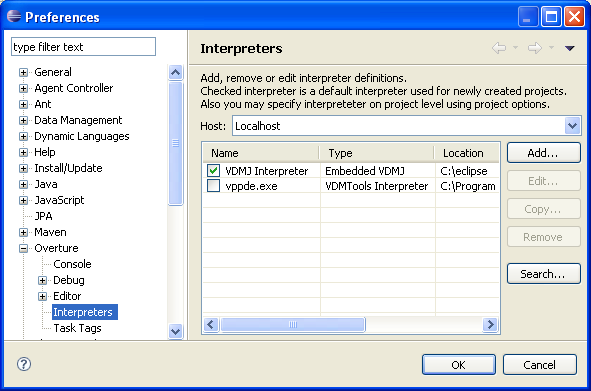
\includegraphics[width=280px]{figures/PreferencesInterpreters}
  \caption{Choosing interpreter}
  \label{fig:userguide:PreferencesInterpreters}
\end{center}
\end{figure}

If one wishes to use VDMJ just enable the 'check box' at VDMJ, for the VDMTools
interpreter click the add\ldots button and choose the VDMTools interpreter and
the path to the executable file to VDMTools.

\subsection{Creating a New Overture Project}
\begin{enumerate}
	\item Create a new project by choosing File $\rightarrow$ new $\rightarrow$
	Overture Project 
	\item Type in a project name
	\item Select dialect type: \textbf{VDM++} 
	\item Chose an interpreter type \textbf{VDMJ} or \textbf{VDMTools} and click
	the finish button see \ref{fig:CreateProjectWizard}
\end{enumerate}

\begin{figure}[!h]
	\begin{center}
	  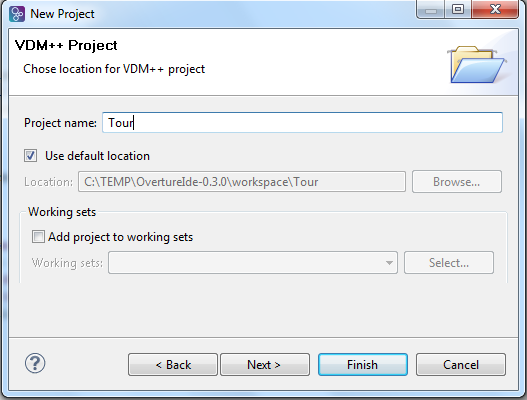
\includegraphics[scale=0.8]{figures/CreateProjectWizard}
	  \caption[Create Project Wizard]{Create Project Wizard}
	  \label{fig:CreateProjectWizard}
	\end{center}
\end{figure}

\framebox{
\begin{minipage}[t]{1\columnwidth}%
	\textbf{Note}: At the moment It doesn't matter which dialect and interpreter
	that is chosen. The dialect VDM++ will always be used.
\end{minipage}}

%%%%%%%%%%%%%%%%%%%%%%%%%%%%%%%%%%
%  Creating a new file
%%%%%%%%%%%%%%%%%%%%%%%%%%%%%%%%%%

\subsection{Creating Files}

Switching to the Overture perspective will change the layout of the user
interface to focus on the VDM development. To change perspective go to the menu 
window $\rightarrow$ open perspective $\rightarrow$ other\ldots and choose the
Overture perspective.
When the developer is in the Overture Perspective the user can create files
using one of the following methods:

\begin{enumerate}
  \item Choose file $\rightarrow$ new $\rightarrow$ VDM File 
  \item Right click on the overture project choose new $\rightarrow$ Overture File 
\end{enumerate}

\section{Overture Perspective}

Figure~\ref{fig:userguire:OverturePerspective} shows the different views
available when editing a model. Each view will be explained in this section.  

\begin{figure}[!h]
\begin{center}
  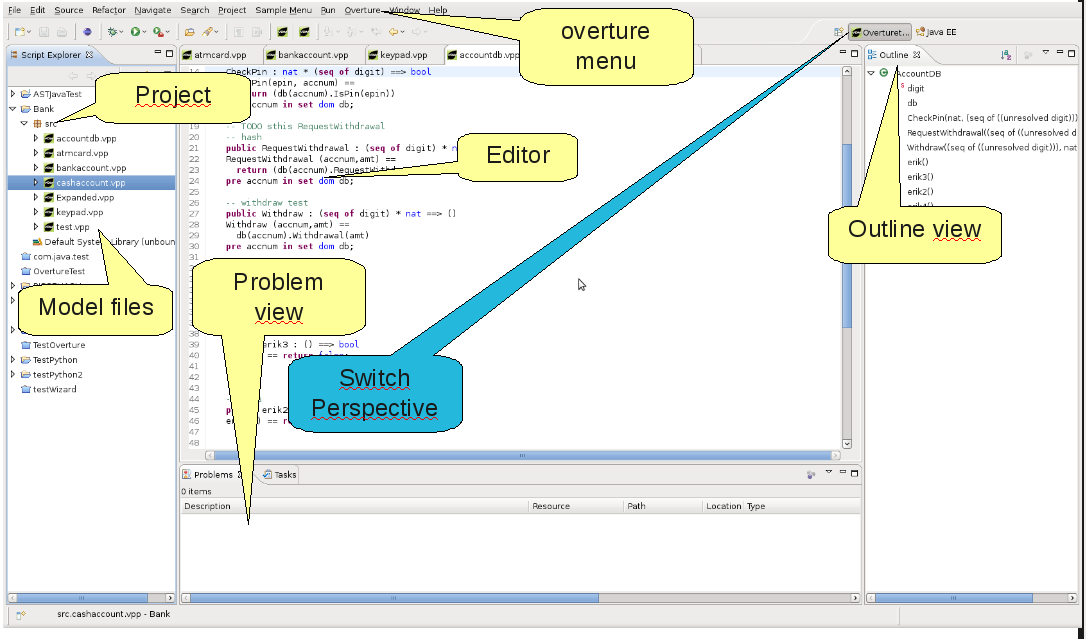
\includegraphics[clip,scale=0.6]{figures/OverturePerspective}
  \caption[labelInTOC]{The Overture Perspective}
  \label{fig:userguire:OverturePerspective}
\end{center}
\end{figure}

\subsection{Project Explorer View}

The Project Explorer View basically provides an overview of projects and
files contained by these projects. double clicking on a model file will open
the file in the Editor.

\subsection{Overture Editor}

The centre of  figure~\ref{fig:userguire:OverturePerspective} shows the Overture
editor, with syntax highlighting. It is possible to change the colour of the
highlighted words, which are divided into groups such as keywords, types, strings
and comments, etc, in the preference page (window $ \rightarrow $ preference $ \rightarrow $
Overture $ \rightarrow $ Editor $ \rightarrow $ Syntax coloring).

The Overture IDE support intellisense, but it is only possible
to complete keywords at the time of writing. The Overture IDE triggers the
proposal when the user hits the key combination \textit{CTRL+space}.  

\subsection{Outline}

The outline view enables the user to navigate quickly in the model,
figure~\ref{fig:userguire:OverturePerspective} shows the outline view at the right
side. A click on a operation/function will move the cursor in the editor to
the definition of the operation. At the top of the outline view there
is a number of buttons which gives the user the option to filter what
is displayed in the outline view, for instance it is possible to hide
variables.

When editing a model, it can be useful to navigate to a specific operation in the
file, instead of reaching for the mouse, this can be done using a shortcut
(Ctrl+O)) which opens a small pop-up. This pop-up allows the user to navigate to
a given location in the model simply by filling out the name of an field,
operation, function or type. The use of intellisense furthermore ensures that the
user does not have to write out the full name of the desired location. Figure
\ref{fig:userguide:quickOutline} shows the quick outline.

\begin{figure}
	\begin{center}
	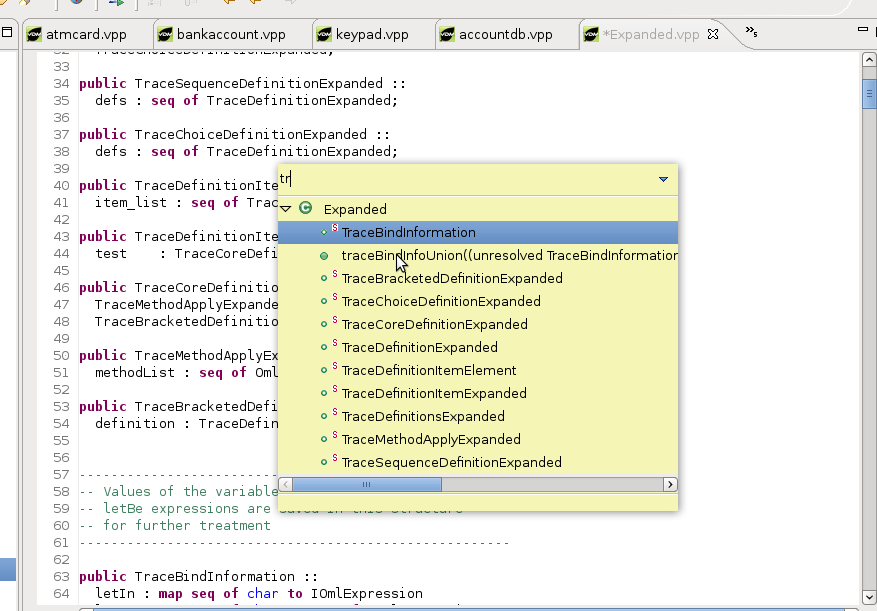
\includegraphics[width=300px]{figures/quickOutline}
	\caption[Quick Outline]{Quick Outline}
	\label{fig:userguide:quickOutline}
	\end{center}
\end{figure}

\subsection{Problems View}

When editing a specification the Overture IDE will parse the content
of the file, if there are any parse errors, it will be reported in
the problems view. See bottom of figure \ref{fig:userguire:OverturePerspective}.
Each time a specification is saved the editor type checks the model
and reports any errors or warnings.

\section{Debugging}

This section describes how to debug a model using the Overture IDE. 

\subsection{Debug configuration}

Debugging the model under development is done by creating a debug configuration
from the menu Run $ \rightarrow  $ Debug configuration\ldots The debug
configuration dialog requires the following information as input to start the
debugger: the project name, the class, the starting operation/function and the
file containing the starting operation/function.
Figure~\ref{fig:userguide:debugConfiguration} shows a debug configuration,
clicking one of the browse buttons will open a dialog which give the user a list
of choices. The class and operation/function are chosen from the dialog with the
list of expandable classes, if the operation or function have arguments these
must be typed in manually.

\begin{figure}[htp]
\begin{center}
  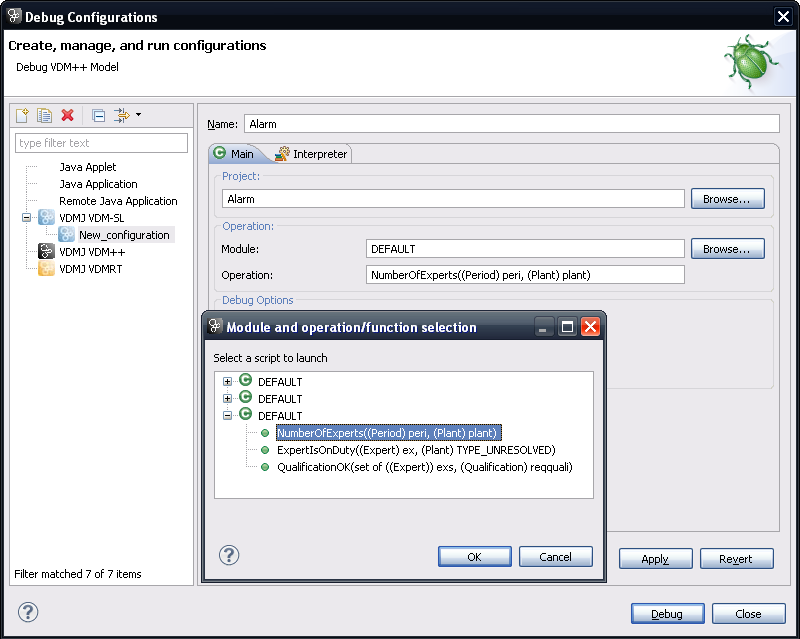
\includegraphics[width=380px]{figures/debugConfiguration}
  \caption{The debug configuration dialog}
  \label{fig:userguide:debugConfiguration}
\end{center}
\end{figure}

\subsection{Debug Perspective}

The Debug Perspective contains the views needed for debugging in VDM. Breakpoints
can easily be set at desired places in the model, by double clicking in left
margin. When the debugger reaches the location of the breakpoint, the user can
inspect the values of different identifiers and step through the VDM model line
by line.
 
The debug perspective shows the VDM model in an editor as the one used in the
Overture Perspective, but in this perspective there are also views useful during
debugging. The features provided in the debug perspective are described below.
The Debug Perspective is illustrated on figure~\ref{fig:userguide:DebuggingVDM}

\begin{figure}[htp]
\begin{center}
  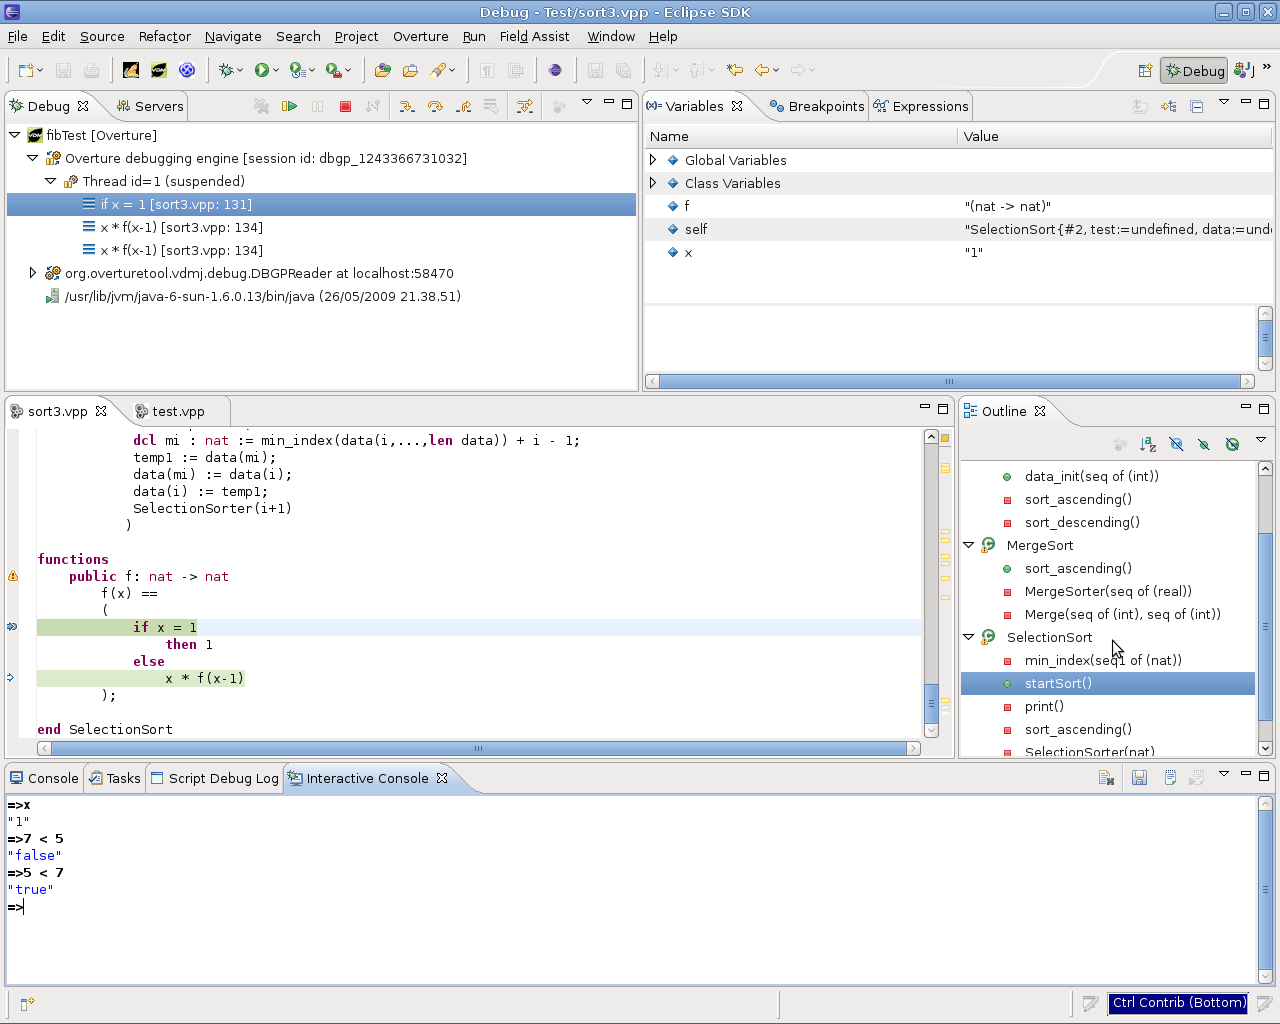
\includegraphics[width=380px]{figures/DebuggingVDM}
  \caption[Debugging perspective]{Debugging perspective}
  \label{fig:userguide:DebuggingVDM}
\end{center}
\end{figure}


\subsubsection{Debug View}
The debug View is located in the upper left corner in the Debug Perspective -
see figure \ref{fig:userguide:DebuggingVDM}. The debug view shows all running
models and the call stack belonging to them. It also displays whether a given model is
stopped, suspended or running. In the top of the view buttons
for debugging such as; stop, step into, step over, resume, etc.\ are located.
All threads are also shown, along with their running status. It is possible to
switch between threads from the Debug View.

\subsubsection{Variables View} 
This view shows all the variables in a given context, when a breakpoint is
reached. The variables and their values displayed are automatically updated when
stepping through a model. The variables view is by default located in the upper
right hand corner in the Debug Perspective. It is also possible to inspect complex variables,
expanding nested arrays and so forth.

\subsubsection{Breakpoints View}
Breakpoints can be added both from the edit perspective and the debug perspective
from the editor view. In the debug perspective however, there is a breakpoints
view that shows all breakpoints. From the breakpoints view the user can easily
navigate to the location of a given breakpoint, disable, delete or set the hit
count or a break condition. In figure \ref{fig:userguide:DebuggingVDM} the
Breakpoints View is hidden behind the Variables View in the upper right hand 
corner in a tabbed notebook. Section~\ref{sec:userguide:breakpoints} explains
how to use conditional breakpoints.

\subsubsection{Expressions View}

The expressions view allows the user to write expressions, as for the
variables view, the expressions are automatically updated when stepping.
Watch expressions can be added manually or created by selecting 'create watch
expression' from the variables view. It is of course possible to edit existing
expressions. Like the Breakpoints View this view is hidden in the upper right
hand corner.

\subsubsection{Interactive Console View}

While the Expressions View allows to easily inspect values, the functionality is
somewhat limited compared with the functionality provided by VDMTools. For more
thorough inspections the Interactive Console View is more suited. Here commands
can be executed on the given context, i.e.\ where the debugger is at a
breakpoint. The Interactive console keeps a command history, so that already
executed commands can be run again without actually typing in the command all
over. Figure~\ref{fig:userguide:interactiveConsole} shows the interactive
console.

\begin{figure}[htp]
\begin{center}
  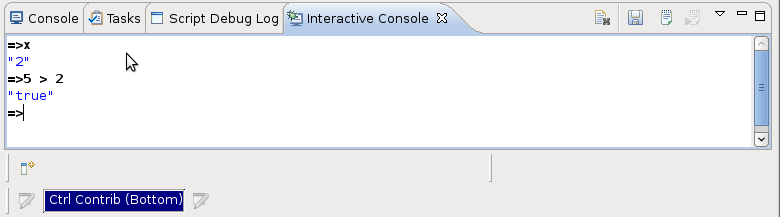
\includegraphics[width=300px]{figures/InteractiveConsole}
  \caption{The interactive console}
  \label{fig:userguide:interactiveConsole}
\end{center}
\end{figure}

\subsubsection{Conditional breakpoints}
\label{sec:userguide:breakpoints}

Conditional breakpoints can also be defined. These are a powerful tool for the
developer since it allows specifying a condition for one or more variables which
has to be true in order for the debugger to stop at the given breakpoint. Apart
from specifying a break condition depending on variables, a hit count can also be
defined. A conditional breakpoint with a hit count lets the user specify a given
number of calls to a particular place at which the debugger should break.

Making a breakpoint conditional is done by right clicking on the breakpoint
mark in the left margin and select the option Breakpoint properties\ldots This
opens a dialog like the one shown in
figure~\ref{fig:userguide:BreakpointConditional}. It is possible to choose
between two different conditional breakpoints, a hit count condition and one
based on an expression defined by the user. 

\begin{figure}[htp]
\begin{center}
  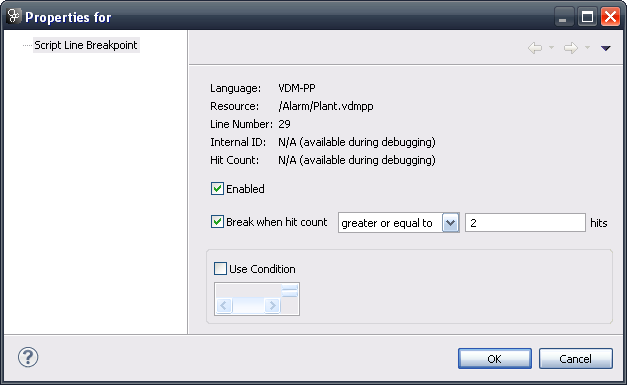
\includegraphics[width=250px]{figures/Breakpointconditional}
  \caption{Conditional breakpoint options}
  \label{fig:userguide:BreakpointConditional}
\end{center}
\end{figure}

\section{Combinatorial Testing}

A specific manual for this topic exist, please refer to \cite{CTManual}.
